\documentclass{article}
\usepackage{graphicx}
\usepackage[margin=1.5cm]{geometry}
\usepackage{amsmath}

\begin{document}

\title{Lab Activity: Pendulum and Energy Conservation}
\author{Prof. Jordan C. Hanson}

\maketitle

\section{Introduction}
A pendulum (Fig. \ref{fig:pend}) is a device that teaches us two things: 1) how to measure $g$ accurately, without dropping anything (and incidentally, how to build a clock), and 2) that energy is conserved. Let $\theta$ be the angle with respect to vertical in Fig. \ref{fig:pend}.
\begin{figure}[ht]
\centering
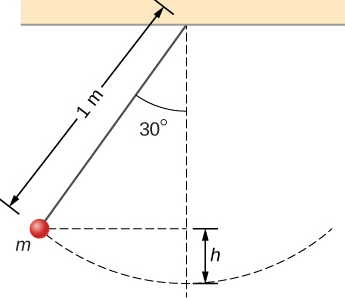
\includegraphics[width=0.2\textwidth]{pend.png}
\caption{\label{fig:pend} A particle hung from a string constitutes a simple pendulum.}
\end{figure}

\section{The Period}

Draw the free body diagram for the case when the pendulum is at its lowest height.  Let $L$ be the length of the pendulum.  Equate the tension with centripetal force, and show that if tension balances gravitational weight, then
\begin{equation}
T = 2\pi \sqrt{\frac{L}{g}}
\end{equation}
Obtain the following: a string and weight, motion sensor, Vernier LabPro device, and a ruler.  Create a pendulum from the weight and string.  Use the motion sensor to measure the period, or time between swings, of the pendulum.  Measure the period for 10 different lengths of the pendulum.  Use Excel to plot $T$ versus $\sqrt{L}$, and fit a trendline.  What is the slope?  How do you extract $g$ from the slope? \\ \vspace{2cm}
\section{Energy Conservation}
Use energy conservation to show that the maximum speed of the weight, for a given initial angle $\theta$ is
\begin{equation}
v_{\rm max} = \sqrt{2gl(1-\cos\theta)} \label{eq:pend}
\end{equation}
Using the motion sensor, measure $v_{\rm max}$ and test whether or not it obeys Eq. \ref{eq:pend}.  If the initial angle is $\theta$, why does the final angle also equal $\theta$?  Do you observe this to be true?
\end{document}